\documentclass{article}
\usepackage{amsmath}
\usepackage{amssymb}
\usepackage{tabularx}
\usepackage{amsmath}
\usepackage{graphicx}
\usepackage{systeme}
\usepackage{nameref}
\usepackage{caption}
\usepackage{url}
\usepackage{float}
\graphicspath{ {./diagrams/} {./screens/} {./official/} }

\begin{document}
\setlength{\parindent}{0in}

\begin{titlepage}
\begin{center}

\begin{large} 
\textsc{Politecnico di Milano}
\end{large}
\\
Scuola di Ingegneria Industriale e dell’Informazione \\
Computer Science and Engineering \\
Dipartimento di Elettronica, Informazione e Bioingegneria \\

\vspace{0.8cm}
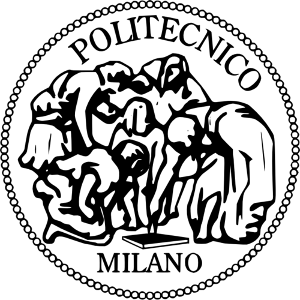
\includegraphics[width=0.4\textwidth]{poli}

\vspace{3cm}

\begin{Large}
\textbf{Asymmetrical multiplayer videogame}
\end{Large}

\vspace{3cm}

\begin{flushleft}
Relatore:
Prof. Marco Gribaudo
\end{flushleft}

\vspace{1cm}

\begin{flushright}
Tesi di Laurea di: \\
Jacopo Grandi, Matr. 947077
\end{flushright}

\vfill
Anno Accademico 2020/2021
\end{center}
\end{titlepage}

\clearpage

\begin{abstract}
Games can be a powerful tool to improve the player's mental and physical skills. The skills we are interested in training are speed of communication, planning and problem solving. They are useful in situations such as a bomb defusal, cave rescues and thick fog navigation, where a team needs remote support to make good decision. We designed and implemented a complete videogame with asymmetrical multiplayer in order to train such skills.
\end{abstract}

\clearpage

\tableofcontents

\clearpage

\section{Introduction}
\subsection{Efficent communication skill development}
The game is focused in training the communication, planning and problem solving skills of the players. The games puts the players under time pressure and requires a significant amount of information to be exchanged quickly. The game also forces a half duplex communication protocol emulating a radio, such that only one player may speak at a time. Some players will also have to solve space navigation puzzles, obstacle avoidance and local route planning; others will have to make a general plan, assign tasks and deal with multitasking.
\subsection{Applicable scenarios}
This skills are useful in environments where the team has no way to take decisions based on their local space and has to rely on another team that has the global picture to make decision for them. Examples of scenarios in such enviroments are cave exploration or cave rescues, firefighting operations in thick fog, bomb defusal and warfare operations. 
\subsection{Feedback on skill improvements}
This is the data gathered from testers.

\clearpage

\subsection{Similar Games}
\subsubsection{Keep Talking and Nobody Explodes}
The game consists in defusing a ticking bomb by solving puzzles attatched to it. It's a two player game, one player is the defuser and the other has a bomb-defusal manual. The players have to exchange the puzzle state and solutions. 

\vspace{0.4cm}
\frame{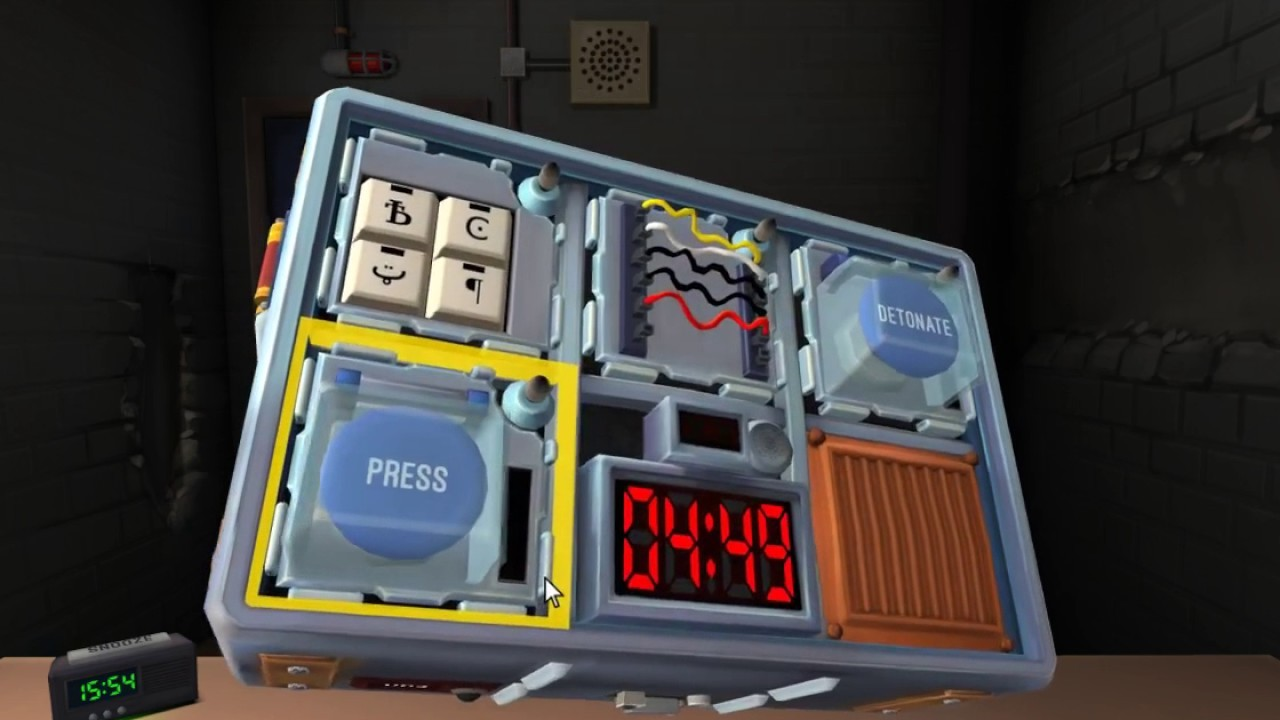
\includegraphics[width=\textwidth]{keep_talking_game}}

\vfill
\frame{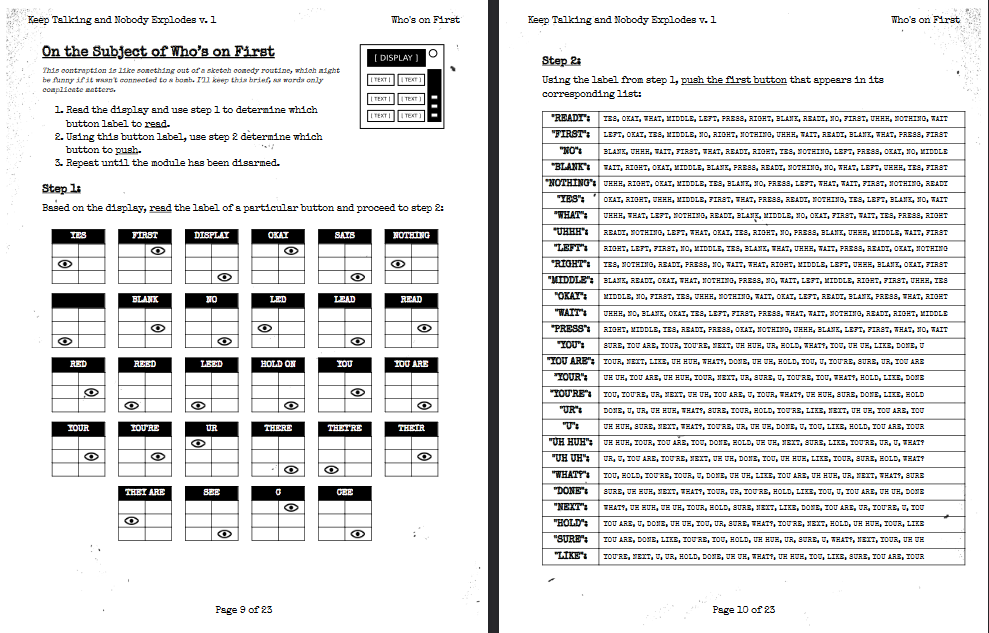
\includegraphics[width=\textwidth]{keep_talking_manual}}

\clearpage

\subsubsection{Unrailed}
The game consists in constructing a railway in front of a moving train. If the trains runs out of track, the game is over. In order to construct rails, the players have to chop trees, mine stone and combine materials in a specialized train cart. It's a 2 to 4 player game. The players  usually talk to split tasks among themselves and get time-sensitive tasks done quickly.

\vspace{0.4cm}
\frame{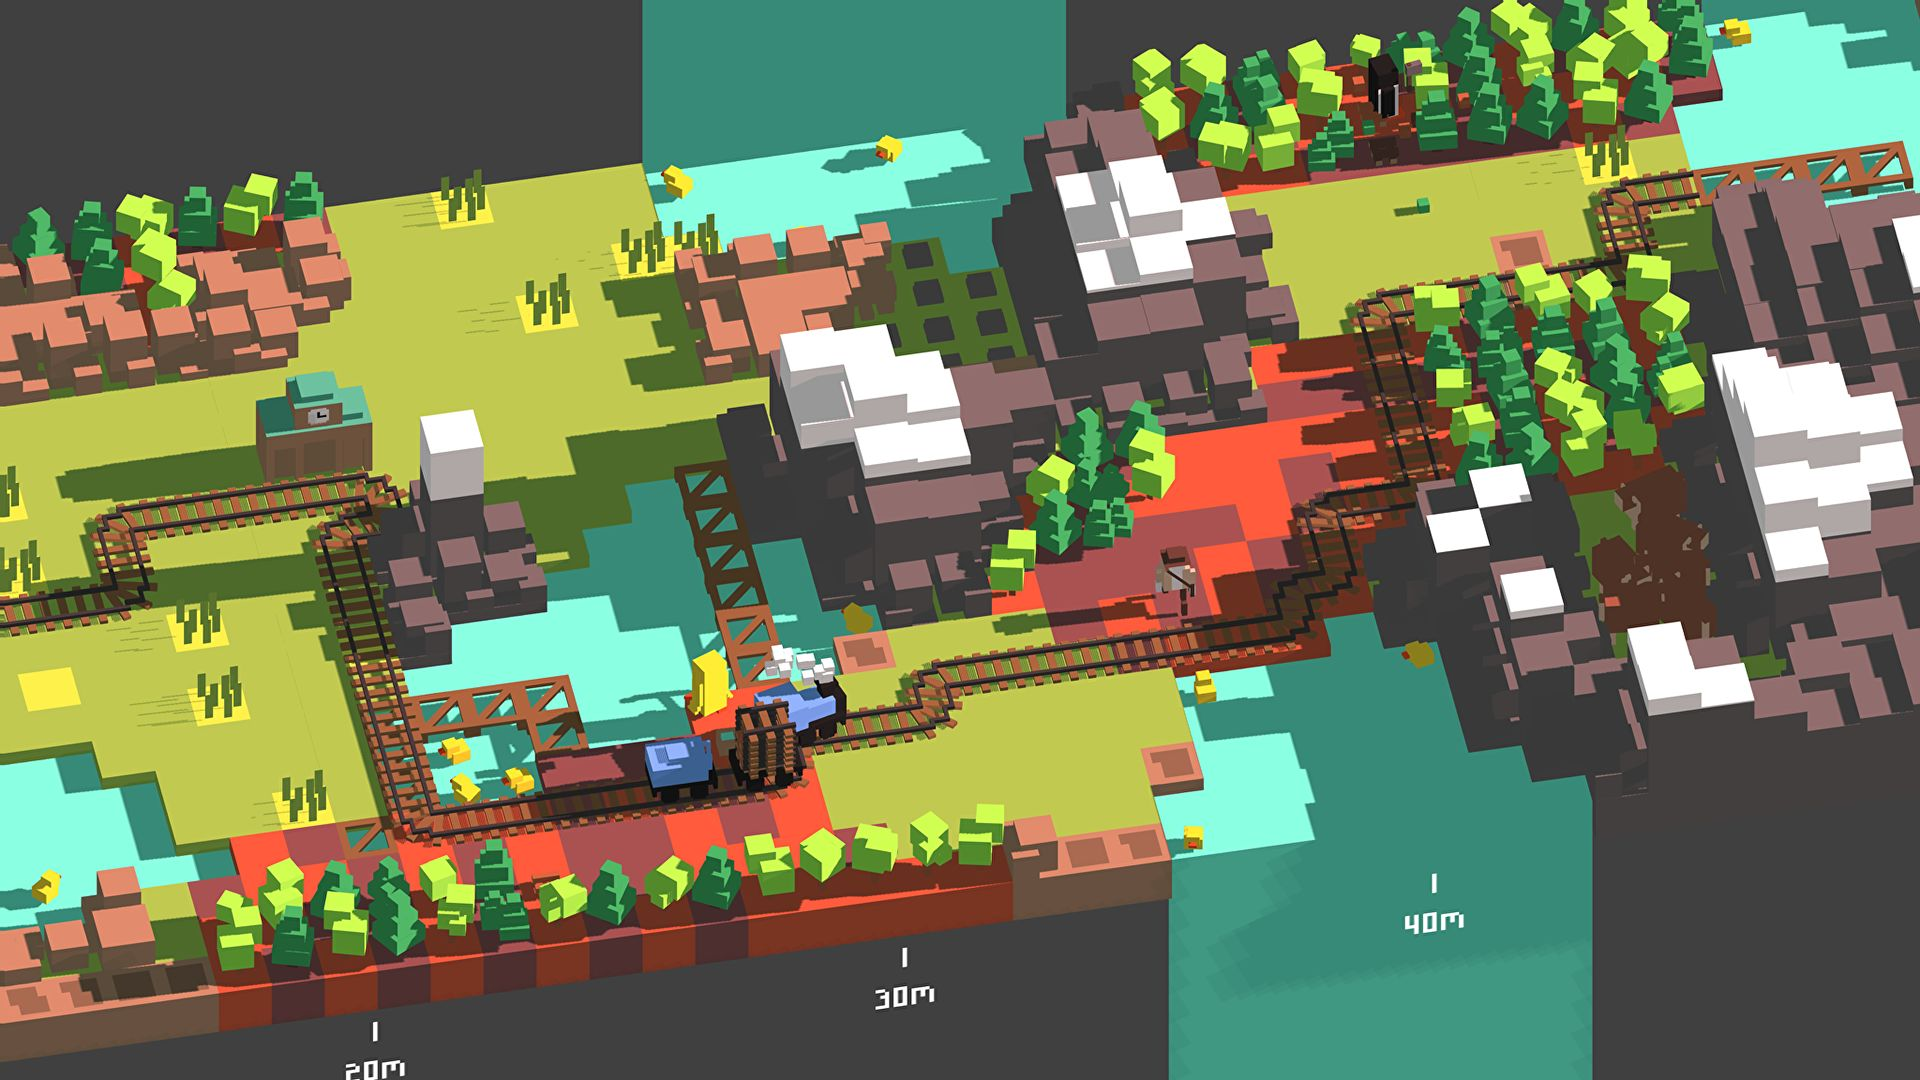
\includegraphics[width=\textwidth]{unrailed}}

\vspace{0.4cm}
The game includes pickups, scattered in the map and difficult to get. This pickups are used to upgrade the train and wagons. The upgrade screen is cooperative too.

\vfill
\frame{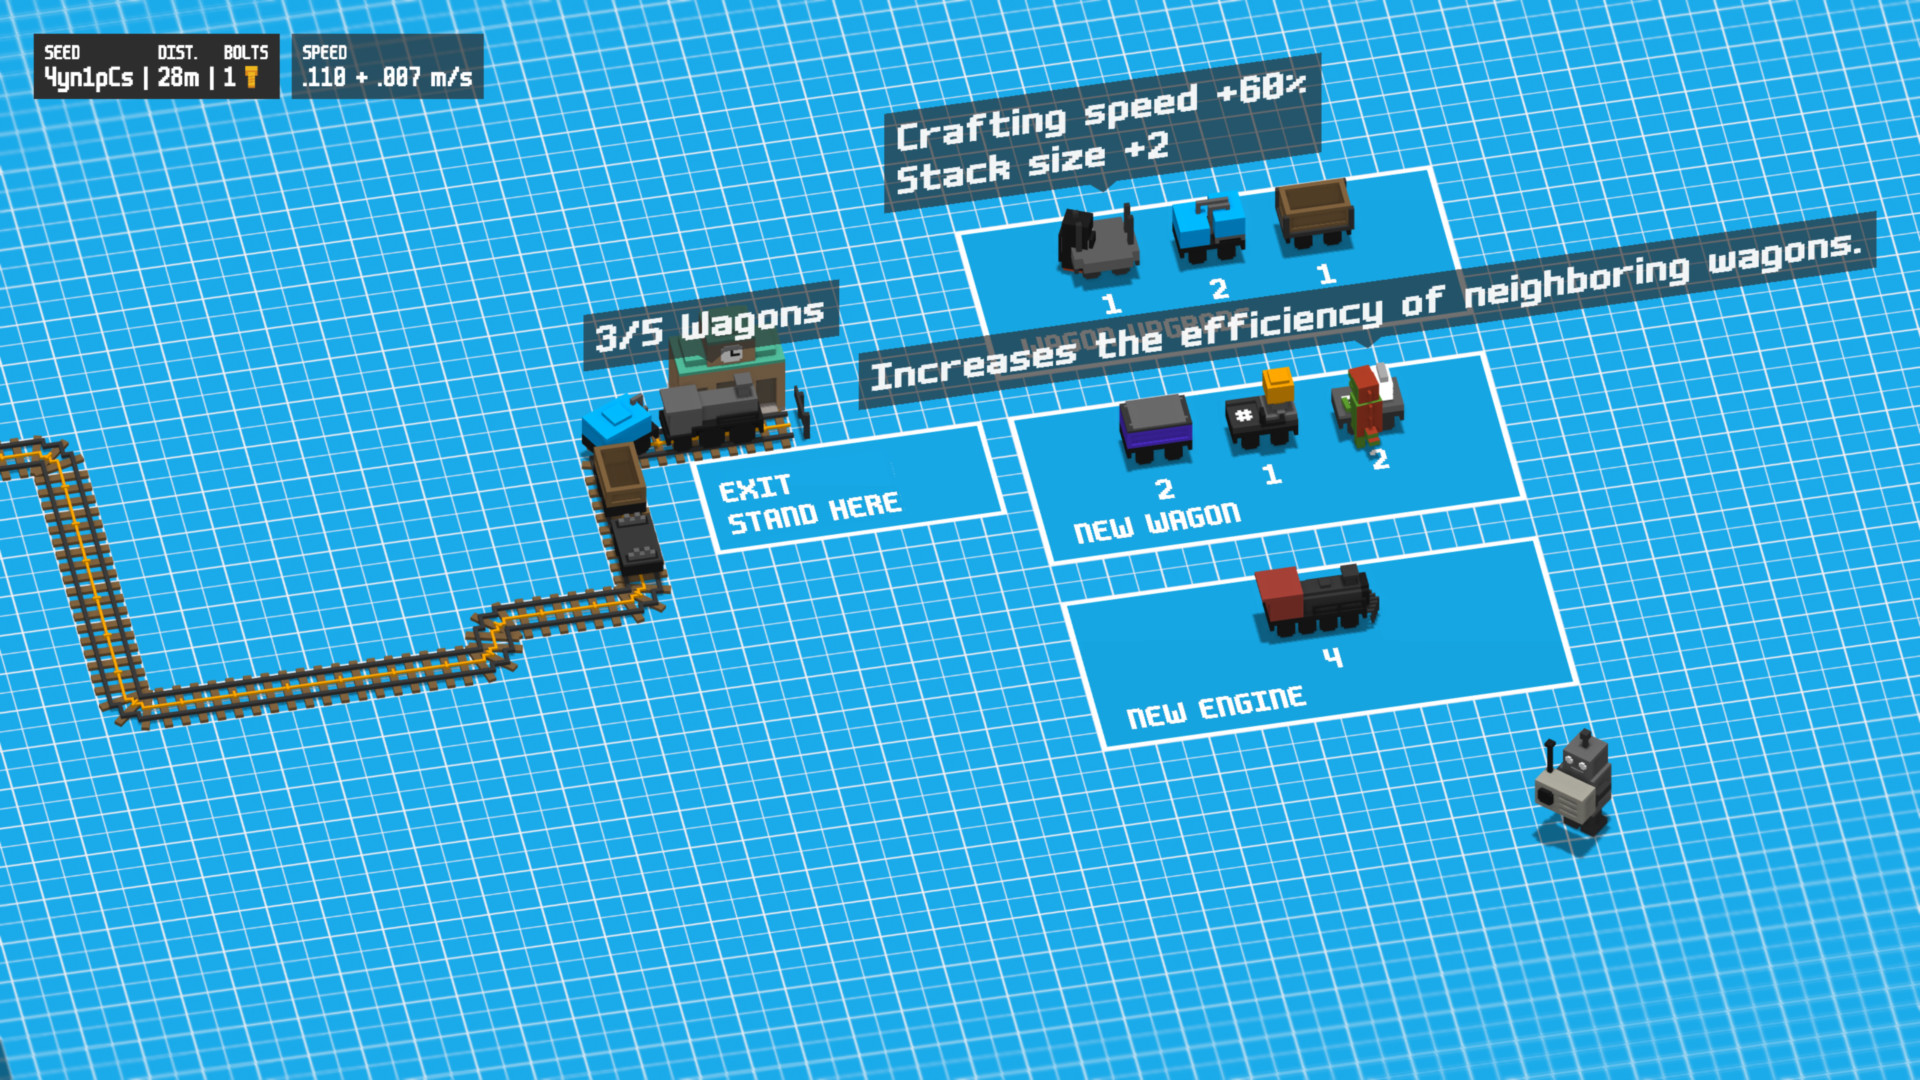
\includegraphics[width=\textwidth]{unrailed_upgrade}}

\clearpage

\subsubsection{Among Us}
This game is a mafia game between two teams, impostors and crewmates, which has become recently popular. A team wins if the other team is dead, crewmates also win when they complete all tasks. Impostors have to kill crewmates. If a crewmate finds a corpse, he may call a vote. The player who has to most votes is killed. The players have to discuss who to kill in a limited time.

\vspace{0.4cm}
\frame{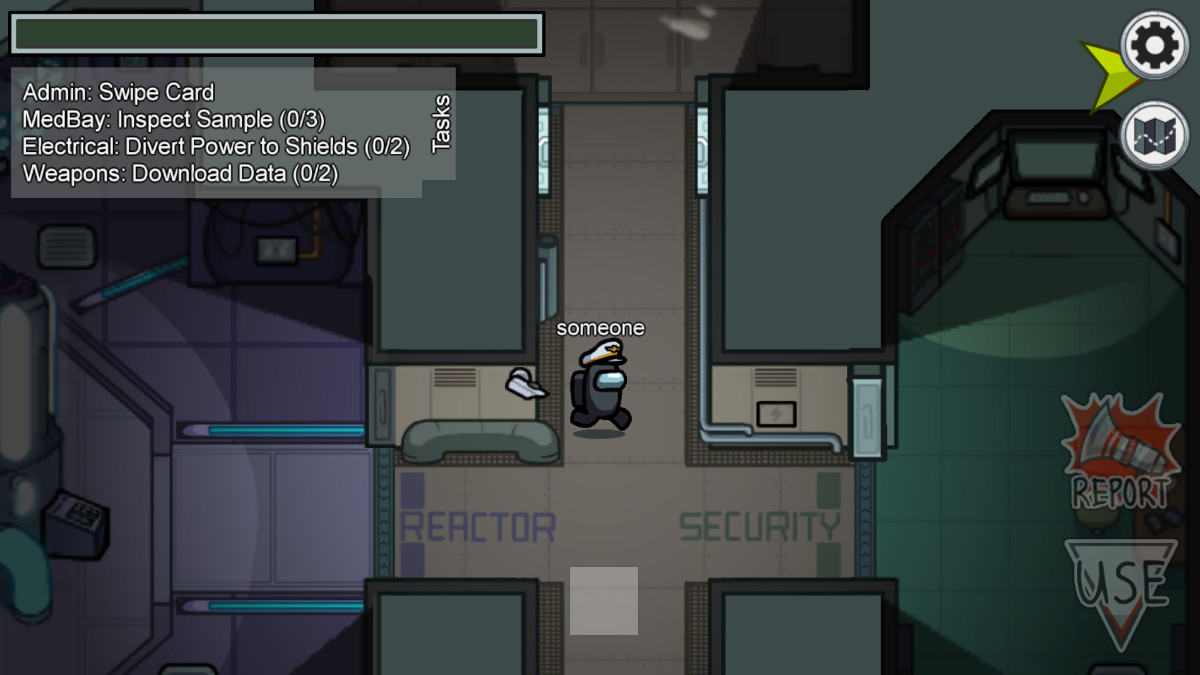
\includegraphics[width=\textwidth]{amongus}}

\vspace{0.4cm}
A player once a game can call an emergency meeting, which triggers the vote without the need to report a corpse.

\vfill
\frame{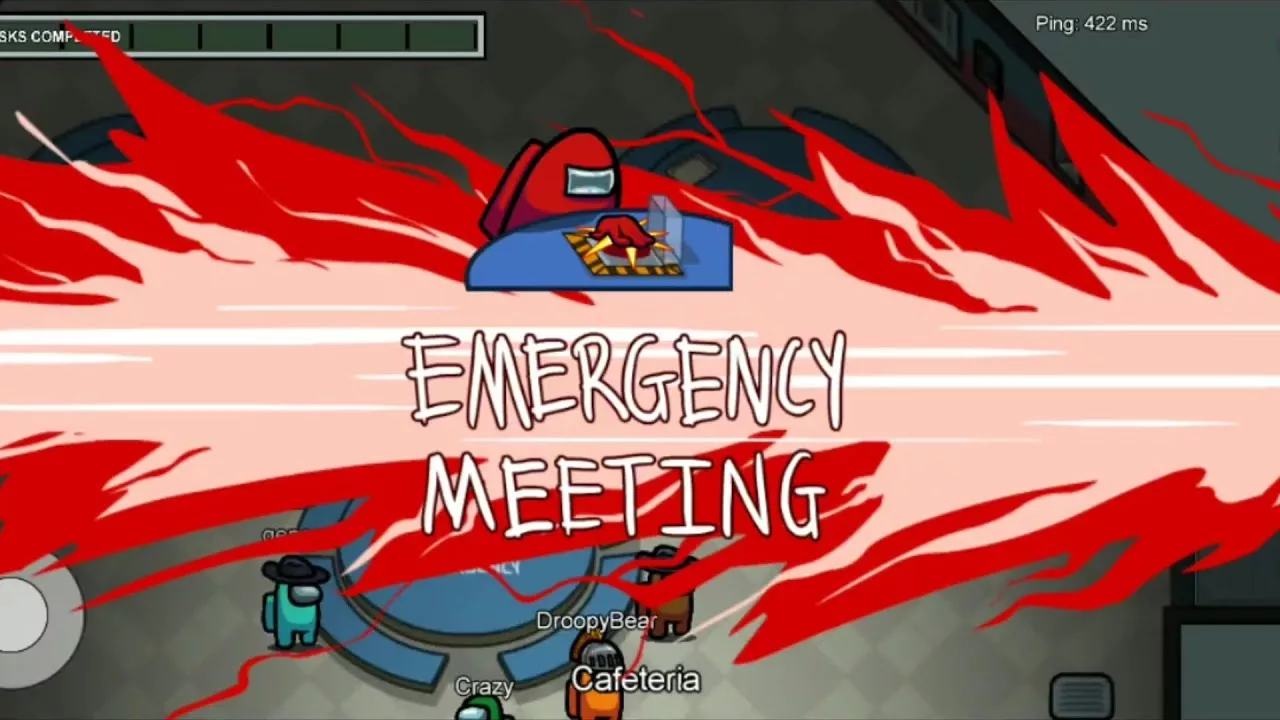
\includegraphics[width=\textwidth]{amongus_meeting}}

\clearpage

\subsection{Asymmetrical Multiplayer}
A game has asymmetrical multiplayer when the players play the game differently. There are multiple levels of asymmetry: from a slight imbalance in the mechanics to a completely separate set of rules. Keep Talking and Nobody Explodes is the most asymmetrical game in the cited games: a player just has a manual. The other two games have a lesser degree of imbalance: in Unrailed the roles and tasks can be exchanged during the games and in amongus every player is controlling a character and interacting in the game's map.

\clearpage

\section{Game Design}
The game is set in a city, with gridstyle roads.
There are up to 2 couriers, which have to fulfil a list of delivery orders.
There is a master player who has a map, which shows the courier's positions and the streets status. The master has the order list, the couriers do not.
The orders consist of a pickup site and dropoff site.
The streets are blocked by many obstacles:
\begin{itemize}
  \item variable level of traffic makes the street difficult to navigate
  \item a drawbridge over a river or a rail
  \item a rail passage getting closed when a train crosses
\end{itemize}
The master has to plan the route during the time and relay the path to each courier in the broadcast channel.
The master's map is outfitted with a shortest path algorithm to ease finding a fast route.
The couriers drive following the Master path, they only see the pickup points and if they have picked up an item, the corrisponding dropoff point.

\subsection{Traffic simulation}
\label{sec:traffic_sym_design}
The traffic simulation can be tuned to different levels of complexity.
\subsubsection{Static}
The streets are filled with a random amount of immoble cars.
\subsubsection{Dynamic}
Every street has a traffic level associated to it. The traffic levels oscillate smoothly following a sine wave with randomized period and phase. The cars are immoble, but when they are not seen by any players, the amount of cars in a street is adjusted to be proportional to the traffic level of the street.
\subsubsection{Agent Based}
The cars are agents that move thorugh a graph representation of the streets. The cars roam through the city by turning randomly at intersections. The cars respect traffic lights and obstacles on the streets, so that traffic jams happen dynamically.

\subsection{Game Variations}
\subsubsection{Events}
Throughout the city there are billboards and signs that contain the time and place an event will happen. The event (for example a parade, a festival, the street market, a strike) generates a lot of foot traffic and car traffic in a particular place. The master has no information about these events, so he has to rely on the couriers who will see the billboards and relay the information.
\subsubsection{Delivery Timers}
The delivery orders may have up to three additional timers: a time after which the order is failed if it's not picked up, a delivery time constraint and a time after which the order is failed if not completed.

\subsection{Master's Information}
The information that the master has of the players can be reduced in the settings. The master has three channels of information: geolocalization, video feed and audio from the radio. Turning off any of these channels the game becomes significantly harder, except when turning off the radio. The radio is essential for completing the game, so it cannot be switched off. A chatting system may substitute it partially.

\subsection{Interface Design}
TODO

\clearpage

\section{Implementation}

\subsection{UDP Sockets with packet fragmentation}
The connection is handled using native C\# asynchronous UDP sockets. The message is sent with a protocol number, a serial identifier that identifies the packet and an id string that identifies the sender. If the message is longer than 1024 bytes, it's fragmented in parts no longer than 1024. Each part has the protocol, the serial number and the id along with an offset and a size. The offset is what part of the original is sent and the size is the size of the whole message. At the receiving end, the datagrams received are assembled back into the original messages using the serial number, the offset and size. The partial messages are stored in a dictionary indexed by the serial number and are made available externally only when full. 
\begin{figure}[H]
\includegraphics[width=\textwidth]{example-image-a}
\caption{Network packet composition}
\end{figure}
\begin{figure}[H]
\includegraphics[width=\textwidth]{example-image-a}
\caption{Message fragmentation}
\end{figure}

\subsection{Model View Controller}
\begin{figure}[H]
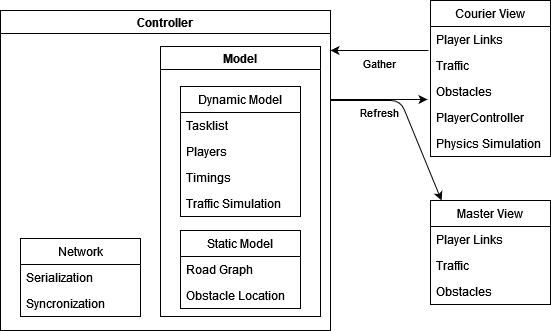
\includegraphics[width=\textwidth]{game architecture}
\caption{Game architecture diagram}
\label{fig:gamearch}
\end{figure}

\subsection{Syncronization model}
The game's state is split in static state and dynamic state. The static state is comprised of the data that does not change during the game and thus is syncronized only at the start of the game. The dynamic state instead is all the data that needs to be syncronized every tick. 
Every tick, which are a few milliseconds apart, each client sends their position to the server. The server integrates the positions in it's state and computes the next state, which is sent back to the clients.
 This approach has the advatage that it's naturally resilient to packet loss as the whole state is sent each time. Moreover, there is no network lag on the client character.
 The approach however has the disadvantage that it's weak against cheating, as the server trusts the position given by the client. This can be solved by running the simulation on the server to check for anomalies or by running it exclusively on the server, gathering the raw inputs of the clients instead of the position.
\smallskip
\begin{figure}[H]
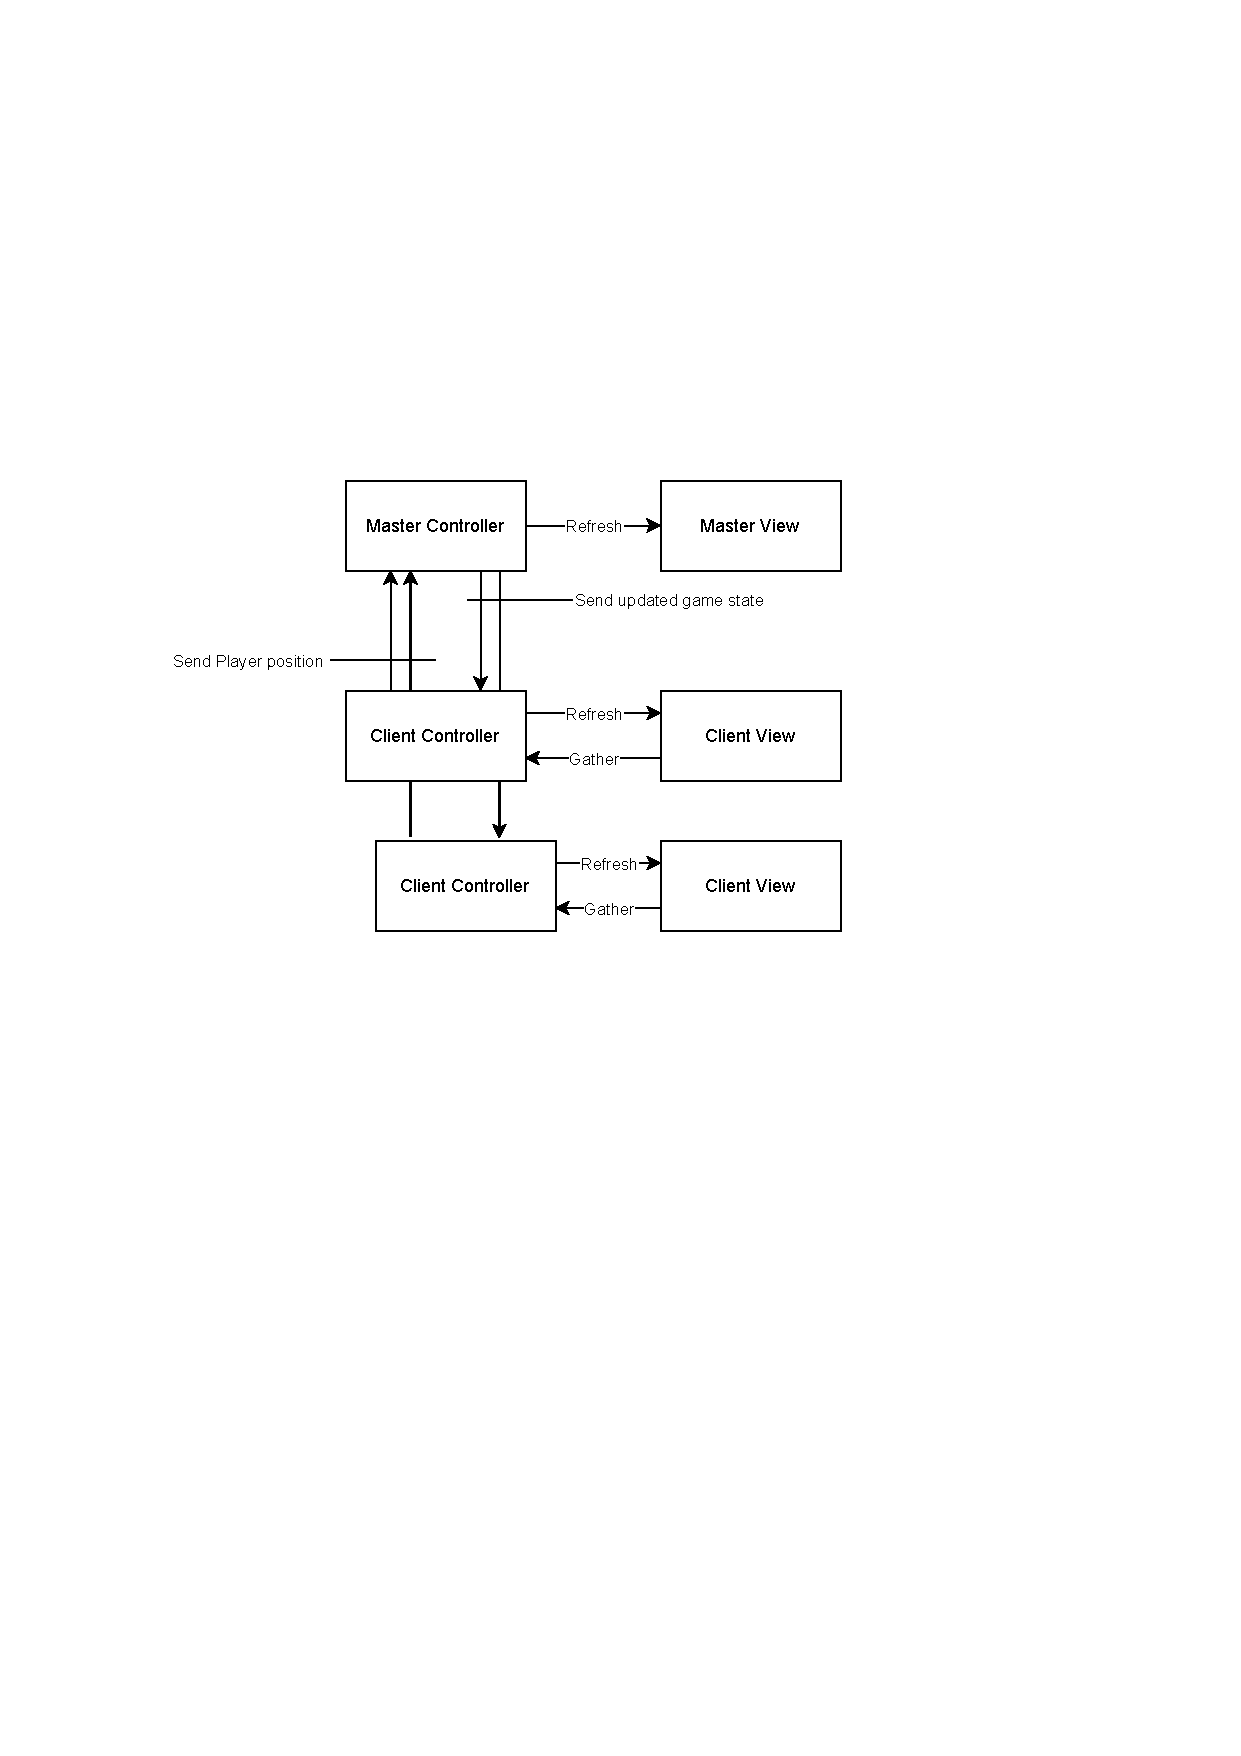
\includegraphics[width=\textwidth]{net architecture}
\caption{Network Architecture diagram}
\end{figure}
\smallskip
The static state is constructed by using the configuration of the lobby. In the lobby of the game, the master has the possibility to change map, set the number of tasks, set the available time and  turn off video feed and geolocalization. The changes are seen by all clients.

\subsubsection{Dead reckoning and latency hiding}
TODO

\clearpage

\subsection{Kinematic Bycicle Model \cite{kbm}}
The model is a simplified car steering model, where the front and back wheels are collapsed into one front wheel and one back wheel. The only steering wheel is the front one. \\
\smallskip
Known constants:
\begin{center}
\( l_r \) = distance from the center to the rear wheel \\
\( l_f \) = distance from the center to the front wheel \\
\end{center}
State variables:
\begin{center}
\( [x, y] \) = absolute position of the bycicle in the plane. \\
\( v \) = velocity of the bicicle. \\
\( \psi \) = heading angle \\
\end{center}
Control variables:
\begin{center}
\( u_1 \) = acceleration \\
\( u_2 \) = steering angle of the front wheel. \\
\end{center}
\begin{figure}[!h]
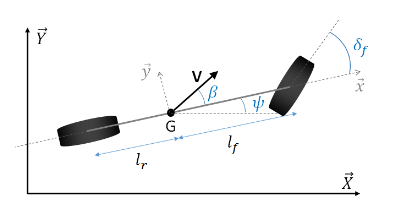
\includegraphics[width=\textwidth]{bike}
\caption{Kinematic bicycle model}
\end{figure}
\smallskip
The model's differential equations:
\begin{equation}\dot{x} = v \cos(\psi + \beta (u_2)) \end{equation}
\begin{equation}\dot{y} = v \sin(\psi + \beta (u_2)) \end{equation}
\begin{equation}\dot{v} = u_1 \end{equation}
\begin{equation}\dot{\psi} = \frac{v} {l_r} \sin(\beta(u_2)) \end{equation}
\medskip
where \( \beta(u_2) \) is the slip angle given by
\begin{equation} \beta(u_2) = \arctan (\tan(u_2) \frac{l_r} { l_f + l_r })  \end{equation}
\bigskip
The model is integrated discretely.
\begin{equation} x_{t+1} = x_t + \dot{x}\Delta t \end{equation}
\begin{equation} y_{t+1} = y_t + \dot{y}\Delta t \end{equation}
\begin{equation} {\psi}_{t+1} = {\psi}_t + \dot{\psi}\Delta t\end{equation}

\clearpage

\subsection{Agent Based Traffic Simulation}
While the static and dynamic (As defined in section~\ref{sec:traffic_sym_design} \nameref{sec:traffic_sym_design}) traffic simulations are straightforward, the agent based one is more difficult to define, relies on more assumptions and is more complex to implement.

\subsubsection{Definition and Assumptions}
The agents of the simulation "cars" are defined by their position relative to a graph, a velocity and other paramters (random acceleration, random seed). This graph called "rail graph" is derived from the street level graph, which is a graph that defines the layout of the roads. The rail graph gets it's name from the cars behaving more like trains or trams, as they cant deviate from the rail graph edges. The rail graph is constructed by replacing every node of the street graph with an intersection and every edge with lanes. The street graph has a parameter for every edge indicating how many lanes the street has.
\begin{figure}[H]
\includegraphics[width=\textwidth]{example-image-a}
\caption{Rail Graph construction from the Street Graph}
\end{figure}
\bigskip 
 The rail graph is directed and the direction of an edge is the direction of the flow of traffic. At the intersection the rails are connected by bezier curves. The left turn rails are not connected to not allow cars to turn left, as it causes a jam instantly.
\begin{figure}[H]
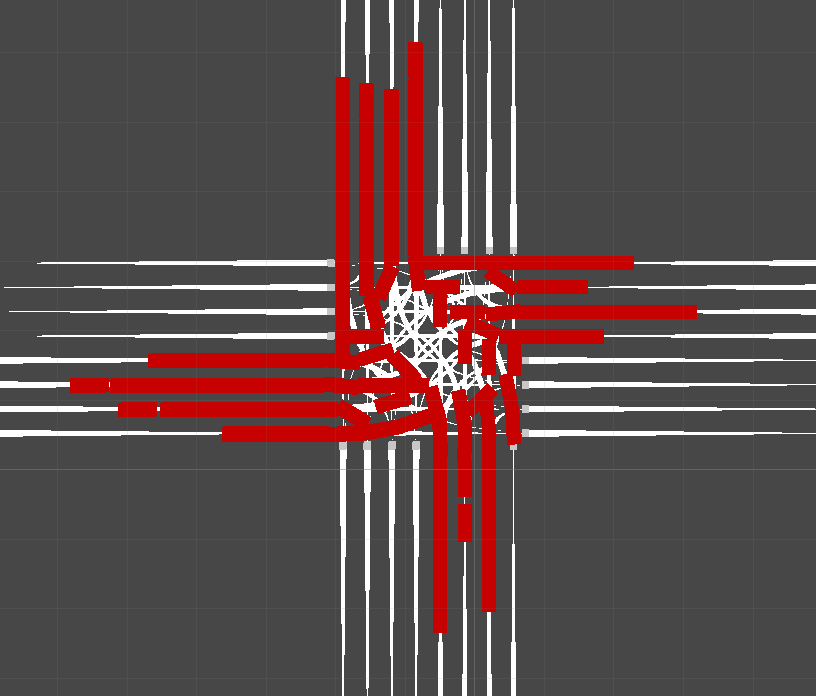
\includegraphics[width=\textwidth]{gridlock}
\caption{Left turn without traffic lights causes instant jam, this is the state after only 10 steps}
\end{figure}
\bigskip 
 To alleviate this jam, the left turning rails would have to be non intersecting and a left turn semaphore would have to be put in place. However, it is not necessary to do so as every point is still reachable without turning left.
Traffic lights are placed on the intersection's inward rails. This lights are coordinated at a street node level, so every semaphore in an intersection is controlled by a single timer. Based on the position of this timer, the semaphores states is set.
\begin{figure}[H]
\includegraphics[width=\textwidth]{example-image-a}
\caption{Semaphore timer and states}
\end{figure}

\subsubsection{Car-Train Agent}
The car's position is defined by the starting node, the ending node (so the edge on which the car is) and the relative position \begin{math}{rel \in [0, 1]}\end{math} along the edge. The absolute position of a car is the position of the car within the frame of reference of the position of the nodes of the rail graph.\\
To get the absolute position a linear interpolation based on the relative position from the start to the end node is performed. If the edge on which the car is on is a bezier, the position is just the evaluation of the equation at the car's relative position.\\
To get the absolute direction the normalized difference of the end and start node is sufficient for the linear case. In the bezier case, the derivative of the bezier equation is the tangent vector, which normalized gives the absolute direction.
\begin{figure}[H]
\includegraphics[width=\textwidth]{example-image-a}
\caption{From the relative position of a car to the absolute position and direction. Left: linear, Right: quadratic bezier}
\end{figure}

\subsubsection{Integration}
The traffic state is a collection of cars. The state is integrated discretely with a time differential dt. Every car calculates how much distance it has to move by using it's velocity. This distance is then consumed by navigating the graph. The car's relative position is incremented by the relative distance, which is the distance divided by the edge length. This is easily calculated for linear edges, but bezier edges have a complex elliptical integral to solve to get their lenght. Therefore, the relative distance is calculated using an approximation of the bezier lenght by sampling a few points. \\
When a car reaches an intersection, if it has a red semaphore it stops. Otherwise, it chooses a rail based on it's initial random seed, which doesn't compromize the deterministic property of the simulation.

\subsubsection{Collision Detection:  Lookahead dictionary}
Before the cars are moved, a lookup dictionary is constructed. This lookahead dictionary stores for every car the position it would have had if it moved some integration steps. The number of lookahead steps is a sensitive parameter with respect to number of incidents and runtime speed. Every time a car is moved, it checks if it would intersect any other future cars using the lookahead dictionary. If it would intersect, the car is stopped. \\
The intersection between two cars is an overlap check on two circles per car that approximate the bounds of a car.

\subsubsection{Lookup optimization and caching}
Every collection used in the simulation can be accessed randomly in constant time and the absolute position and direction of a car are recalculated only when the relative position is modified. The rail graph has precalculated structures such as an index for accessing edges directly and a forward star collection for every node.

\subsubsection{Intersection optimization: Grid indexing}
The intersection checking is the most costly operation for the simulation. In order to check faster, the cars further than a radius are excluded from the check. This is a coarse filter, but it requires a quadratic number of checks w.r.t. the number of cars. Therefore, an index based on the car's position is implemented. This index divides the space in a grid and for every square it has a collection listing all cars contained in the square. This index can be queried to return a neighbor of a car, and it does so by returning all cars in the original car square and all adjacent squares. 

\subsubsection{Parallel Integration}
The integration and collision detection algorithm can operate on a copy of the traffic state (which is a dictionary of cars) and apply the changes at the end of computation thanks to the lookahead dictionary. This makes it possible to parallelize the creation of the lookahead dictionary, the position integration and the collision detection. The threads have access to all the indexed data and traffic state and place their result into thread-safe containers. The threads work on a subset of cars and can't contaminate each other subset as they are changed at the end of computation.

\subsubsection{Stopped cars linking optimization}
The cars which are traveling and detect a still car on their path are stopped and linked to the other car. This link is broken when the car detects that the linked car is moving. When a car is linked to another, it's not needed in the lookahead dictionary and can skip being moved. \\
This linking procedure helps speeding up the intersection check, which is the slowest part of the whole simulation. Although, in the initial state the cars are placed in such a way that no car is linked, which forces the simulation to run slower until some cars are stopped in order for the linking procedure to take effect.

\subsubsection{Traffic Syncronization}
TODO

\clearpage

\subsection{Radio}
The radio in the game is a simulation of a real half-duplex radio. This means that only one player at the time may speak. This is enforced by transmitting white noise while two ore more player are using the radio channel simultaneously. The simulation relies on a server based network to centralize the audio mixing process. All clients send their audio to the server, which mixes all the sources and sends customized mixes to each client and the local speaker. As a convention, all audio passing though the mixer has a sampling rate of 48kHz. 
\subsubsection{Voice Loopback}
The client audio doesn't loop back to the sender. When the voice returns to the speaker it's delayed, causing confusion. The server processes all audio sources to calculate if noise is needed, then for every client it mixes all sources except the client one.
\subsubsection{Buffers}
The client audio is sent to the server and cached in a buffer in order to account for desyncronizations and network jitters. The server creates and fills a buffer for every client. Periodically, the server polls the buffers and mixes the polled data. The mix is sent to each client where it is cached in a buffer. This buffer is constantly polled by an Unity audio callback. The draining and filling of the buffers is balanced: the microphones produce as many samples as the ones consumed by the speakers, so the intermediate buffers serve as a transfer node. 
\begin{figure}[H]
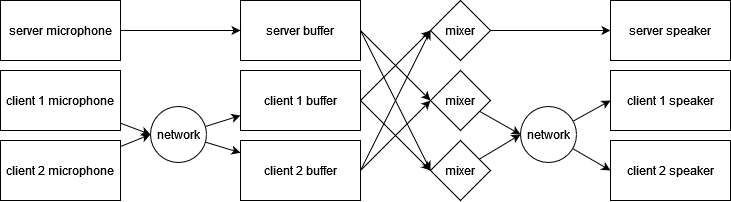
\includegraphics[width=\textwidth]{audio mixer}
\caption{Audio pipeline diagram, the boxes represent the buffers.}
\end{figure}
Every buffers delays the signal by a set amount. This delay is crucial to alleviate the network variance, which otherwise would cut the signal and override samples. The buffers, when queried to read a certain amount of data, return silence if the data available is less than the requested amount. This ensures that the mixer will always have either a full set of data or silence and that the buffers will not cut the audio.

\clearpage

\subsubsection{Sampling frequency and Resampling}
The client's microphone may have a different sampling frequency from each other. The audio sent is resampled to 48 kHz and the audio received is resampled to the speakers sampling frequency. The sampler used is a custom sample and hold algorithm, it inserts or deletes samples following the ratio of sample rates.
\subsubsection{Noise and Filters \cite{filters}}
The noise generated and mixed when multiple clients are speaking is white noise at 48 kHz. The audio generated by the clients is filtered by the server with a custom hi pass filter, which attenuates the low frequencies. This effect is done to make the simulation closer to an old style radio.\\
\begin{figure}[H]
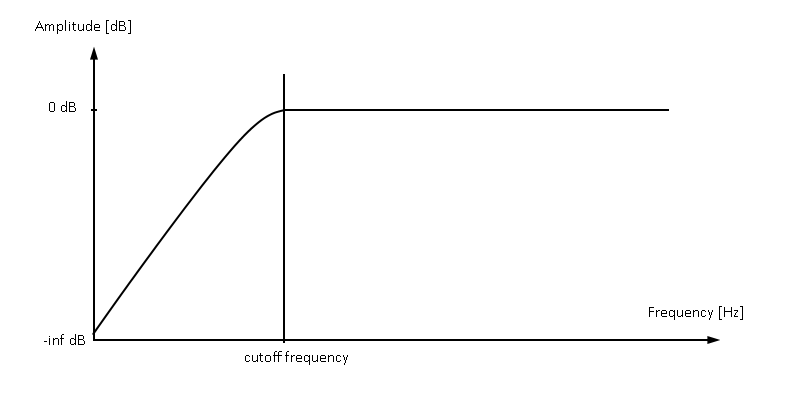
\includegraphics[width=\textwidth]{hipass}
\caption{Hi-Pass filter Bode diagram}
\end{figure}
\bigskip
The filter is a recursive digital filter, defined by the following differential equation:
\begin{equation} y(n) =\alpha (y(n-1) + x(n) - x(n-1))\end{equation}

\subsection{Video}
The video feed is a frame of the player's camera which is sent to the master by each player. The amount of data required scales rapidly with the resolution of the frame and the frequency of the transmission.

\subsection{Editor Tools}
The development process was sped up by the construction of tools for Unity. This tools are based on editor scripts, which allows to automatize some actions in the editors such as instantiating prefabs (keeping the prefab link) and destroying GameObjects.
\subsubsection{Map Generator}
The map generator places prefabs on a grid, randomizes their z rotation snapping on the 4 cardinal rotations and swaps these prefabs with their updated ones. This script also places road segments ensuring that no segment overlaps another and giving each segment a unique identifier.
\subsubsection{Graph Generator}
This tool generates a graph (a nodes and arcs tuple) from the elements present in the scene. The graph is saved directly in the Assets/Resources folder in json format. The graph can be visualized in the scene with a toggle in the script. The tool also visualizes the traffic rail graph, the cars and the traffic lights state. The traffic simulation can be stepped through directly in the unity editor, which eliminates the need to wait for unity to reset it's state while entering play mode.

\subsection{Unity Optimizations}
Culling, LODs, events
TODO

\clearpage

\section{Testing}
\subsection{Unit Testing}
Unit tests are automated tests, they ensure that a small section of code behaves as intended. It's difficult to write testable code and to write tests for all the required functionality if the tests are not included in the design. To make it easier to write a complete test suite (set of tests of a program), a tecnique called test driven development is used to write code and tests.
\subsubsection {Test Driven Development \cite{tdd}} 
The model of the game is developed using the test driven development technique. This technique allows writing testable code by first writing a failing test and then the code to pass it. This makes the code more robust and easier to clean. Other aspect of the game such as the controller, the view or the map tools are not easily testable this way as they depend on the unity framework. One of the goals of TDD is to make it easy to refactor code: if the refactored code passes all tests the code is correct, there's no need to run it to know. This relies on the robustness of the test suite. If an essential functionality is not tested, the test suite is incomplete and by running all tests there is no guarantee of correctness.
\subsection{Integration Testing}
The integration testing phase is largely done by hand. This is necessary as unity does't have a way to run multiple deployed instances inside a test environment. The testing routine is to deploy an executable and run it parallel to the editor instance. Some components are tested automatically, such as the serialization of the model and the interaction between smaller model components.
\subsection{Clumsy \cite{clumsy}}
Clumsy is a program that makes the internet network worse. It simulates packet loss, jitter, latency, bandwith problems, it tampers with packets. This tool is the basis on the game's retransmission algorithm, because it creates the perfect network conditions for testing.

\clearpage
\bibliographystyle{plain}
\bibliography{references}

\end{document}